\documentclass[tikz,border=2mm]{standalone}
\definecolor{structure}{HTML}{1A535C}   % Deep Teal
\definecolor{main}{HTML}{C6892A}       % Golden Ochre
\definecolor{second}{HTML}{2E4057}     % Slate Blue
\definecolor{third}{HTML}{8B2635}      % Burgundy
\usetikzlibrary{positioning}

\begin{document}

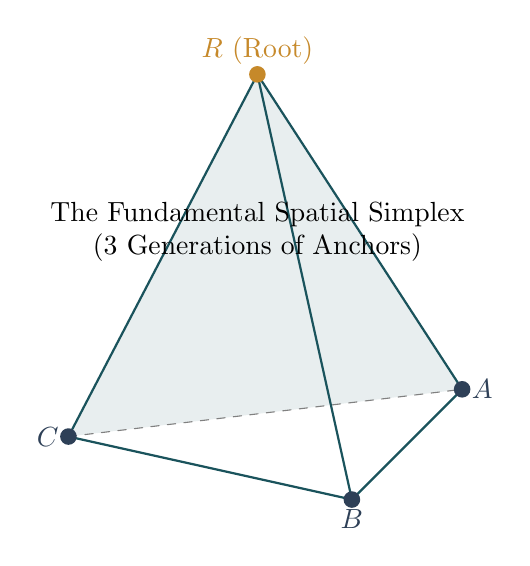
\begin{tikzpicture}[scale=2, line join=round, line cap=round]
    % Coordinates for Tetrahedron (3-simplex)
    \coordinate (A) at (1.5, -0.5);   % Anchor A
    \coordinate (B) at (0.8, -1.2);   % Anchor B (front)
    \coordinate (C) at (-1, -0.8);    % Anchor C
    \coordinate (R) at (0.2, 1.5);    % Root event (top vertex)

    % Back face (R-C-A) — shaded for depth cue
    \fill[structure!10] (R) -- (C) -- (A) -- cycle;

    % Hidden edge (dashed)
    \draw[dashed, thin, gray] (C) -- (A);

    % Visible edges
    \draw[thick, structure] (R) -- (C);
    \draw[thick, structure] (R) -- (A);
    \draw[thick, structure] (R) -- (B);
    \draw[thick, structure] (C) -- (B);
    \draw[thick, structure] (B) -- (A);

    % Vertex labels
    \fill[main]   (R) circle (1.5pt) node[above] {$R$ (Root)};
    \fill[second] (A) circle (1.5pt) node[right] {$A$};
    \fill[second] (B) circle (1.5pt) node[below] {$B$};
    \fill[second] (C) circle (1.5pt) node[left]  {$C$};

    % Caption
    \node[align=center, below=1.5cm of R]
        {The Fundamental Spatial Simplex \\ (3 Generations of Anchors)};
\end{tikzpicture}

\end{document}
